\documentclass[../Main.tex]{subfiles}
\begin{document}
  \chapter{2023-2024学年微积分（一）（下）期中考试}

  \section{基本计算题(每小题 6 分，共 60 分)}
  \begin{enumerate}
    \item 已知$\boldsymbol{a}\times (\boldsymbol{b}\times \boldsymbol{a}) = \boldsymbol
      {b}-2\boldsymbol{a}$，且$|\boldsymbol{a}|=1$，$|\boldsymbol{b}|=4$，求$|\boldsymbol
      {b}+\boldsymbol{a}|$.
      \vspace{10em}

    \item 已知单位向量$\overrightarrow{OA}$与$x$轴正向的夹角为$\frac{\pi}{3}$，与$y$轴正向的夹角为$\frac{\pi}{4}$，且在$z$轴上的坐标是负的.
      $\overrightarrow{OB}=\left(1,-\sqrt{2},-1\right)$，求$\angle AOB$的角平分线上的单位向量.
      \vspace{12em}

    \item 求圆锥面$2x^{2}+2y^{2}-z^{2}=0$与旋转抛物面$z=x^{2}+y^{2}$的交线在$P(1,
      1,2)$处的切线与法平面方程.
      \vspace{12em}

    \item 设$u=f(x,y,z)$具有连续的偏导数，$z=z(x,y)$是由方程$z^{5}-xz^{4}+yz^{3}=
      1$确定的隐函数，其中$5z^{2}-4xz+3y\neq0$，又$f'_{1}(0,0,1)=2$，$f'_{2}(0,0,
      1)=4$，$f'_{3}(0,0,1)=1$，求$\left.\mathrm{d}u\right|_{(0,0)}$.
      \vspace{12em}

    \item 设$z=yf(x^{2}-y^{2})$，其中$f$可导，求$\frac{1}{x}z_{x}+\frac{1}{y}z_{y}$.
      \vspace{12em}

    \item 求积分$I=\int_{1}^{3}\mathrm{d}x\int_{x-1}^{2}\sin y^{2}\mathrm{d}y$.
      \vspace{12em}

    \item 设平面区域$D=\{(x,y)|-2x\leq x^{2}+y^{2}\leq 4\}$，求二重积分$I=\iint\limits
      _{D}\left(y\cos x+\sqrt{x^{2}+y^{2}}\right)\mathrm{d}x\mathrm{d}y$.
      \vspace{12em}

    \item 设有直线$L:
      \begin{cases}
        x+5y+z=0, \\
        x-z+4=0
      \end{cases}$，平面$\pi:x-4y-8z+12=0$，求直线$L$在平面$\pi$上的投影直线的方程.
      \vspace{10em}

    \item 将空间曲线$\begin{cases}
        x^{2}+y^{2}+z^{2}=1,        \\
        (x-1)^{2}+y^{2}+(z-1)^{2}=1
      \end{cases}$化为参数方程.
      \vspace{10em}

    \item 计算三重积分$I=\iiint\limits_{\Omega}\mathrm{e}^{1-z}\mathrm{d}x\mathrm{d}
      y\mathrm{d}z$，其中$\Omega$是三坐标面与平面$x+y+z=1$所围成的四面体.
      \vspace{10em}
  \end{enumerate}

  \section{综合题(每小题 8 分，共 40 分)}
  \begin{enumerate}
    \item[11.] 若函数$u=az^{4}-bxz+x^{2}+y^{2}$在点$P(1,1,1)$处沿方向$\boldsymbol
      {l}=(2,1,2)$的方向导数最大，求$a,b$的值，并求出最大方向导数.
      \vspace{13em}

    \item[12.] 已知函数$f(x,y)=x^{3}+y^{3}-(x+y)^{2}+2$，$D$是由$x+y=3$，$x=0$，$y
      =0$所围成的平面区域，求$f(x,y)$在$D$上的最大值与最小值.
      \vspace{13em}

    \item[13.] 设$z(x,y)=x^{y}+\int_{0}^{x}x\mathrm{e}^{-(y+t)^2}\mathrm{d}t$，求$\left
      .\frac{\partial^{2} z}{\partial x \partial y}\right|_{(1,0)}$.
      \vspace{12em}

    \item[14.] 设$f(x,y)=
      \begin{cases}
        \frac{x^3y}{x^4+y^2}, & x^{4}+y^{2}\neq0, \\
        0,                    & x^{4}+y^{2}=0.
      \end{cases}$讨论函数$f(x,y)$在原点处的连续性、偏导数存在性及可微性.
      \vspace{12em}

    \item[15.] 设函数$f(x),g(x)$在$[0,b]$上连续且单调增加，其中$b>0$，用\textbf{二重积分}证明:
      \[
        b\int_{0}^{b}f(x)g(x)\mathrm{d}x\geq \int_{0}^{b}f(x)\mathrm{d}x\int_{0}^{b}
        g(x)\mathrm{d}x
      \]
      \vspace{10em}
  \end{enumerate}

  \chapter{2023-2024学年微积分（一）（下）期中考试参考答案}
  \section{基本计算题(每小题 6 分，共 60 分)}
  \begin{enumerate}
    \item \textbf{Solution}. 由题意可得
      \[
        \begin{aligned}
          0 = \boldsymbol{a}\cdot \left(\boldsymbol{a}\times (\boldsymbol{b}\times\boldsymbol{a})\right) = & \boldsymbol{a}\cdot (\boldsymbol{b}-2\boldsymbol{a})                                         \\
          =                                                                                                & \boldsymbol{a}\cdot\boldsymbol{b}-2|\boldsymbol{a}|^{2}=\boldsymbol{a}\cdot\boldsymbol{b}-2.
        \end{aligned}
      \]

      所以$\boldsymbol{a}\cdot\boldsymbol{b}=2$.

      $|\boldsymbol{b}+\boldsymbol{a}| = \sqrt{(\boldsymbol{b}+\boldsymbol{a})^{2}}
      = \sqrt{|\boldsymbol{b}|^{2}+|\boldsymbol{a}|^{2}+2\boldsymbol{a}\cdot\boldsymbol{b}}
      = \sqrt{16+1+4}= \sqrt{21}$.

    \item \textbf{Solution}. 设$\alpha,\beta,\gamma$分别为$\overrightarrow{OA}$与$x$轴、$y$轴、$z$轴的夹角，

      则由题意可得$\cos \alpha = \frac{1}{2}$，$\cos \beta = \frac{\sqrt{2}}{2}$.
      因$\cos^{2} \alpha + \cos^{2} \beta + \cos^{2} \gamma = 1$，所以$\cos \gamma
      = \pm \frac{1}{2}$，

      又$\overrightarrow{OA}$在$z$轴上的坐标是负的，所以$\cos \gamma = -\frac{1}{2}$.
      从而$\overrightarrow{OA}= \left(\frac{1}{2},\frac{\sqrt{2}}{2},-\frac{1}{2}
      \right)$.

      $\overrightarrow{OB^0}=\left(\frac{1}{2},-\frac{\sqrt{2}}{2},-\frac{1}{2}\right
      )$，所以$\frac{\overrightarrow{OA}+\overrightarrow{OB^0}}{|\overrightarrow{OA}+\overrightarrow{OB^0}|}
      = \left(\frac{\sqrt{2}}{2},0,-\frac{\sqrt{2}}{2}\right)$.

      即所求的$\angle AOB$的角平分线上的单位向量为$\left(\frac{\sqrt{2}}{2},0,-\frac{\sqrt{2}}{2}
      \right)$.

    \item \textbf{Solution}. 设$F(x,y,z) = 2x^{2}+2y^{2}-z^{2}$，$G(x,y,z)=x^{2}+
      y^{2}-z$.

      \textbf{法一} . 因$\frac{\partial (F,G)}{\partial (y,z)}\bigg|_{P}=
      \begin{vmatrix}
        4y & -2z \\
        2y & -1
      \end{vmatrix}_{P}=\left.-4y+2yz\right|_{P}=4\neq 0$，

      所以方程组$\begin{cases}
        F(x,y,z)=0, \\
        G(x,y,z)=0
      \end{cases}$可以唯一确定两个具有连续导数的隐函数$y=y(x),z=z(x)$.

      方程组$\begin{cases}
        F(x,y,z) = 2x^{2}+2y^{2}-z^{2}=0, \\
        G(x,y,z)=x^{2}+y^{2}-z=0
      \end{cases}$两边对$x$求导，得 $\begin{cases}
        4x+4y\frac{\mathrm{d}y}{\mathrm{d}x}-2z\frac{\mathrm{d}z}{\mathrm{d}x}= 0, \\
        2x+2y\frac{\mathrm{d}y}{\mathrm{d}x}-\frac{\mathrm{d}z}{\mathrm{d}x}= 0.
      \end{cases}$

      解得$\begin{cases}
        \frac{\mathrm{d}y}{\mathrm{d}x} = -\frac{x}{y}, \\
        \frac{\mathrm{d}z}{\mathrm{d}x} = 0
      \end{cases}$，所以切线的方向向量可取为$\left(1,\frac{\mathrm{d}y}{\mathrm{d}x}
      ,\frac{\mathrm{d}z}{\mathrm{d}x}\right)_{P}=(1,-1,0)$，

      切线的方程为$\frac{x-1}{1}=\frac{y-1}{-1}=\frac{z-2}{0}$，

      法平面的方程为$1\cdot(x-1)-1\cdot(y-1)+0\cdot(z-2)=0$，即$x-y=0$.

      \textbf{法二}. $\nabla F = (4x,4y,-2z)$，$\nabla G = (2x,2y,-1)$，

      取两个曲面的法向量分别为$\boldsymbol{n}_{F} = \frac{1}{4}\nabla F|_{P} = (1
      ,1,-1)$，$\boldsymbol{n}_{G} = \nabla G|_{P} = (2,2,-1)$，

      所以切线的方向向量可取为$\boldsymbol{n}_{F}\times \boldsymbol{n}_{G} =
      \begin{vmatrix}
        \boldsymbol{i} & \boldsymbol{j} & \boldsymbol{k} \\
        1              & 1              & -1             \\
        2              & 2              & -1
      \end{vmatrix}
      = (1,-1,0)$，

      切线的方程为$\frac{x-1}{1}=\frac{y-1}{-1}=\frac{z-2}{0}$，

      法平面的方程为$1\cdot(x-1)-1\cdot(y-1)+0\cdot(z-2)=0$，即$x-y=0$.

    \item \textbf{Solution}. 方程$z^{5}-xz^{4}+yz^{3}=1$两边全微分，得
      \[
        5z^{4}\mathrm{d}z-z^{4}\mathrm{d}x-4xz^{3}\mathrm{d}z+z^{3}\mathrm{d}y+3y
        z^{2}\mathrm{d}z=0,
      \]

      将$x=0,y=0,z=1$代入上式，得$5\mathrm{d}z-\mathrm{d}x+\mathrm{d}y=0$.所以
      \[
        \begin{aligned}
          \left.\mathrm{d}u\right|_{(0,0)}= & f'_{1}\mathrm{d}x+f'_{2}\mathrm{d}y+f'_{3}\mathrm{d}z                     \\
          =                                 & 2\mathrm{d}x+4\mathrm{d}y+\mathrm{d}z                                     \\
          =                                 & 2\mathrm{d}x+4\mathrm{d}y+\frac{1}{5}\left(\mathrm{d}x-\mathrm{d}y\right) \\
          =                                 & \frac{11}{5}\mathrm{d}x+\frac{19}{5}\mathrm{d}y.
        \end{aligned}
      \]

    \item \textbf{Solution}. $z_{x} = yf'(x^{2}-y^{2})\cdot 2x$，$z_{y} = f(x^{2}
      -y^{2})+yf'(x^{2}-y^{2})\cdot (-2y)$，

      所以$\frac{1}{x}z_{x}+\frac{1}{y}z_{y} = 2yf'(x^{2}-y^{2})+\frac{f(x^{2}-y^{2})}{y}
      -2yf'(x^{2}-y^{2}) = \frac{f(x^{2}-y^{2})}{y}$.

    \item \textbf{Solution}. 积分区域$D$如右图所示.交换积分次序得
      \begin{figure}[h] % 图片
        \small \raggedleft
        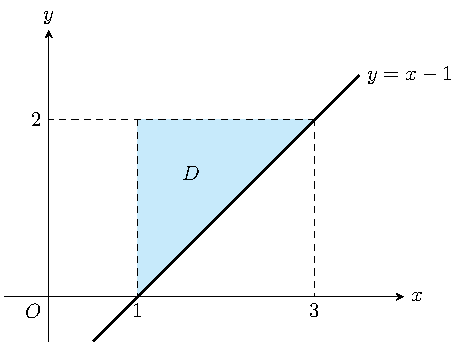
\includegraphics[width=5cm]{2024x-figure1.pdf} % 引入图片源
      \end{figure} % 图片结束
      \vspace{-12.5em}

      $\begin{aligned}
        I = & \int_{1}^{3}\mathrm{d}x\int_{x-1}^{2}\sin y^{2}\mathrm{d}y = \int_{0}^{2}\mathrm{d}y\int_{1}^{y+1}\sin y^{2}\mathrm{d}x \\
        =   & \int_{0}^{2}y\sin y^{2}\mathrm{d}y = \left.-\frac{1}{2}\cos y^{2}\right|_{0}^{2}                                        \\
        =   & -\frac{1}{2}\cos 4 + \frac{1}{2}= \frac{1}{2}(1-\cos 4).
      \end{aligned}$

    \item \textbf{Solution}. 由于积分区域 $D$ 关于 $x$ 轴对称，所以 $\iint\limits
      _{D}y\cos x\mathrm{d}x\mathrm{d}y=0$.

      记 $D'=\{(x,y)|-2x\leq x^{2}+y^{2}\leq 4, y\geq 0\}$，则
      $I = 2\iint\limits_{D'}\sqrt{x^{2}+y^{2}}\mathrm{d}x\mathrm{d}y$.

      用极坐标代换，则

      \noindent
      \begin{minipage}[c]{0.5\textwidth}
        $\begin{aligned}
          I & = 2\iint\limits_{D'}\sqrt{x^2+y^2}\mathrm{d}x\mathrm{d}y                                                                                                               \\
            & = 2\left(\int_{0}^{\frac{\pi}{2}}\mathrm{d}\theta\int_{0}^{2}r^{2}\mathrm{d}r+\int_{\frac{\pi}{2}}^{\pi}\mathrm{d}\theta\int_{-2\cos\theta}^{2}r^{2}\mathrm{d}r\right) \\
            & = \frac{8}{3}\pi + \frac{16}{3}\int_{\frac{\pi}{2}}^{\pi}\left(1+\cos^{3}\theta\right)\mathrm{d}\theta                                                                 \\
            & = \frac{16}{3}\pi + \frac{16}{3}\int_{\frac{\pi}{2}}^{\pi}\cos^{3}\theta\mathrm{d}\theta                                                                               \\
            & = \frac{16}{9}(3\pi-2).
        \end{aligned}$
      \end{minipage}
      \hfill %
      \begin{minipage}[c]{0.5\textwidth}
        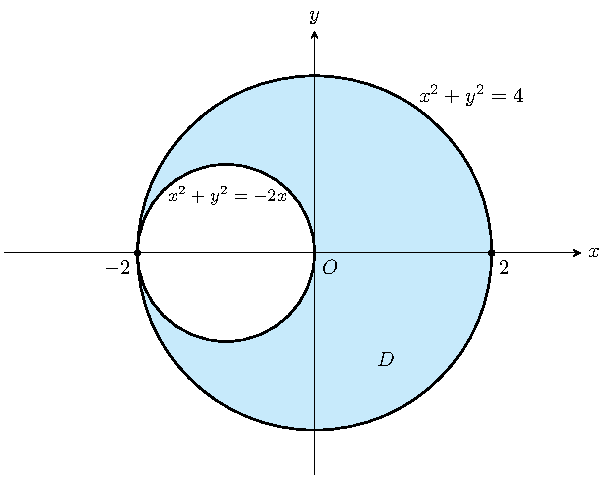
\includegraphics[width=7cm]{2024x-figure2.pdf} % 引入图片源
      \end{minipage}

    \item \textbf{Solution}. 设过直线$L:
      \begin{cases}
        x+5y+z=0, \\
        x-z+4=0
      \end{cases}$的平面束方程为$x+5y+z+\lambda(x-z+4)=0$，

      即$(1+\lambda)x+5y+(1-\lambda)z+4\lambda=0$.

      令其与平面$\pi:x-4y-8z+12=0$垂直，得$(1+\lambda)\cdot 1+5\cdot(-4)+(1-\lambda
      )\cdot(-8) = 0$，解得$\lambda=3$.

      所以直线$L$在平面$\pi$上的投影直线的方程为$\begin{cases}
        4x+5y-2z+12=0, \\
        x-4y-8z+12=0.
      \end{cases}$

    \item \textbf{Solution}. 在方程组$\begin{cases}
        x^{2}+y^{2}+z^{2}=1,        \\
        (x-1)^{2}+y^{2}+(z-1)^{2}=1
      \end{cases}$中消去$y$，得$(x-1)^{2}+(z-1)^{2}=x^{2}+z^{2}$，

      即$x+z=1$.将$z=1-x$代入$x^{2}+y^{2}+z^{2}=1$，得曲线在$xOy$平面上的投影柱面方程：$2
      x^{2}-2x+y^{2}=0$，

      即$4\left(x-\frac{1}{2}\right)^{2}+2y^{2}=1$. 令$\begin{cases}
        x-\frac{1}{2} = \frac{1}{2}\cos \theta, \\
        y = \frac{1}{\sqrt{2}}\sin \theta,
      \end{cases}(0\leq \theta < 2\pi)$，则$z=1-x=\frac{1}{2}-\frac{1}{2}\cos\theta$，

      故曲线的参数方程为$\begin{cases}
        x = \frac{1}{2}+\frac{1}{2}\cos \theta, \\
        y = \frac{1}{\sqrt{2}}\sin \theta,      \\
        z = \frac{1}{2}-\frac{1}{2}\cos \theta.
      \end{cases}(0\leq \theta < 2\pi)$

    \item \textbf{Solution}. 用截面法，
      \[
        \begin{aligned}
          I = \iiint\limits_{\Omega}\mathrm{e}^{1-z}\mathrm{d}x\mathrm{d}y\mathrm{d}z = & \int_{0}^{1}\mathrm{e}^{1-z}\mathrm{d}z\iint\limits_{D_z}\mathrm{d}x\mathrm{d}y \qquad \left(D_{z}=\{(x,y)|x\geq 0,y\geq 0,x+y\leq 1-z\}\right)                               \\
          =                                                                             & \frac{1}{2}\int_{0}^{1}(1-z)^{2}\mathrm{e}^{1-z}\mathrm{d}z = \frac{1}{2}\int_{0}^{1}z^{2}\mathrm{e}^{z}\mathrm{d}z                                                           \\
          =                                                                             & \frac{1}{2}\int_{0}^{1}z^{2} \mathrm{d}\mathrm{e}^{z}= \frac{1}{2}\left(z^{2}\mathrm{e}^{z}\Big|_{0}^{1}-\int_{0}^{1}2z\mathrm{e}^{z}\mathrm{d}z\right)                       \\
          =                                                                             & \frac{\mathrm{e}}{2}-\int_{0}^{1}z\mathrm{e}^{z}\mathrm{d}z = \frac{\mathrm{e}}{2}-\int_{0}^{1}z\mathrm{d}\mathrm{e}^{z}                                                      \\
          =                                                                             & \frac{\mathrm{e}}{2}-\left(z\mathrm{e}^{z}\Big|_{0}^{1}-\int_{0}^{1}\mathrm{e}^{z}\mathrm{d}z\right) = \frac{\mathrm{e}}{2}-\left(\mathrm{e}-\left(\mathrm{e}-1\right)\right) \\
          =                                                                             & \frac{1}{2}\mathrm{e}-1.
        \end{aligned}
      \]
  \end{enumerate}

  \section{综合题(每小题 8 分，共 40 分)}
  \begin{enumerate}
    \item[11.] \textbf{Solution}. $\frac{\partial u}{\partial x}= -bz+2x$，$\frac{\partial
      u}{\partial y}= 2y$，$\frac{\partial u}{\partial z}= 4az^{3}-bx$.

      所以$\nabla u|_{P}= \left.(-bz+2x,2y,4az^{3}-bx)\right|_{(1,1,1)}= (-b+2,2,
      4a-b)$.

      由于函数沿梯度方向的方向导数最大，所以$\nabla u|_{P}//\boldsymbol{l}$，有
      \[
        \frac{-b+2}{2}= \frac{2}{1}= \frac{4a-b}{2},
      \]

      解得$a=\frac{1}{2}$，$b=-2$. 此时$\nabla u|_{P}= (4,2,4)$，所以最大方向导数为$|
      \nabla u|_{P}| = \sqrt{4^{2}+2^{2}+4^{2}}= 6$.

    \item[12.] \textbf{Solution}. 先考虑$D$的内部. 令$f'_{x}= 3x^{2}-2(x+y) = f'_{y}
      = 3y^{2}-2(x+y) = 0$，

      解得唯一驻点$\left(\frac{4}{3},\frac{4}{3}\right)$，$f\left(\frac{4}{3},\frac{4}{3}
      \right)=\left(\frac{4}{3}\right)^{3}+\left(\frac{4}{3}\right)^{3}-\left(\frac{4}{3}
      +\frac{4}{3}\right)^{2}+ 2=-\frac{10}{27}$.

      考虑$D$的坐标轴边界. 由对称性不妨只考虑在$y$轴上时，

      此时$x=0$，$f(x,0) = x^{3}-x^{2}+2$，令$\left(x^{3}-x^{2}+2\right)'=3x^{2}-
      2x=0$，解得$x=0$或$\frac{2}{3}$，

      $f\left(0,0\right) = 2$，$f\left(\frac{2}{3},0\right) = f\left(0,\frac{2}{3}
      \right) = \frac{50}{27}$.

      再考虑$D$的斜边边界，即直线$x+y=3$，

      此时$f = x^{3}+(3-x)^{3}-7$，令$\left(x^{3}+(3-x)^{3}-7\right)' = 3x^{2}-3(
      3-x)^{2}=0$，解得$x=\frac{3}{2}$，

      $f\left(\frac{3}{2},\frac{3}{2}\right) = -\frac{1}{4}$，$f(3,0)=f(0,3) = 20$.

      比较得函数$f(x,y)$在$D$上的最大值为$20$，最小值为$-\frac{10}{27}$.

    \item[13.] \textbf{Solution}. 令$u=y+t$，则$\mathrm{d}u = \mathrm{d}t$，$\int
      _{0}^{x}x\mathrm{e}^{-(y+t)^2}\mathrm{d}t = x\int_{y}^{y+x}\mathrm{e}^{-u^2}
      \mathrm{d}u$.

      所以$z(x,y) = x^{y}+x\int_{y}^{y+x}\mathrm{e}^{-u^2}\mathrm{d}u$，

      $\frac{\partial z}{\partial x}= yx^{y-1}+\int_{y}^{y+x}\mathrm{e}^{-u^2}\mathrm{d}
      u+x\cdot \mathrm{e}^{-(y+x)^2}$，
      \[
        \begin{aligned}
          \frac{\partial^2 z}{\partial x \partial y}= & \frac{\partial}{\partial y}\left(yx^{y-1}+\int_{y}^{y+x}\mathrm{e}^{-u^2}\mathrm{d}u+x\cdot \mathrm{e}^{-(y+x)^2}\right) \\
          =                                           & x^{y-1}+yx^{y-1}\ln x + \mathrm{e}^{-(y+x)^2}-\mathrm{e}^{-y^2}+x\cdot \mathrm{e}^{-(y+x)^2}\cdot (-2)(y+x)              \\
          =                                           & x^{y-1}\left(1+y\ln x\right)+\mathrm{e}^{-(y+x)^2}\left(1-2x(y+x)\right)-\mathrm{e}^{-y^2}.
        \end{aligned}
      \]

      从而$\left.\frac{\partial^{2} z}{\partial x \partial y}\right|_{(1,0)}= -\frac{1}{\mathrm{e}}$.

    \item[14.] \textbf{Solution}. 利用$\left(x^{2}-y^{2}\right)^{2}\geq 0$可得$\left
      |\frac{x^{3} y}{x^{4} + y^{2}}\right| \leq \frac{|x|}{2}$. 所以当$(x,y)\to(
      0,0)$时，$\left|\frac{x^{3} y}{x^{4} + y^{2}}\right| \leq \frac{|x|}{2}\to0$，

      由夹逼定理可知$\lim_{\substack{x\to 0 \\ y\to 0}}\frac{x^{3} y}{x^{4} + y^{2}}
      =0=f(0,0)$，因此函数$f(x,y)$在原点处连续.

      又$f(x,0)=f(0,y)\equiv 0$，所以$f_{x}(0,0)=f_{y}(0,0)=0$，因此函数$f(x,y)$在原点处的偏导数存在.

      考察$\lim_{\substack{x\to 0 \\ y\to 0}}\frac{f(x,y)-f(0,0)-f_{x}(0,0)x-f_{y}(0,0)y}{\sqrt{x^{2}+y^{2}}}
      = \lim_{\substack{x\to 0 \\ y\to 0}}\frac{x^{3} y}{\left(x^{4} + y^{2}\right)\sqrt{x^2+y^2}}$.

      当$y=x^{2},x\to0,y\to0$时，$\lim_{\substack{x\to 0 \\ y\to 0}}\frac{x^{5}}{2x^{4}\sqrt{x^2+x^4}}
      = \lim_{x\to0}\frac{x}{2|x|\cdot\sqrt{x^2+1}}= \frac{1}{2}\lim_{x\to0}\frac{x}{|x|}$不存在，

      所以函数$f(x,y)$在原点处不可微.

    \item[15.] \textbf{Solution}. 记区域$D=\{(x,y)|0\leq x\leq b,0\leq y\leq b\}$，$I
      =b\int_{0}^{b}f(x)g(x)\mathrm{d}x-\int_{0}^{b}f(x)\mathrm{d}x\int_{0}^{b}g(
      x)\mathrm{d}x$，则
      \[
        \begin{aligned}
          I = & \int_{0}^{b}\mathrm{d}y\int_{0}^{b}f(x)g(x)\mathrm{d}x - \int_{0}^{b}f(x)\mathrm{d}x\int_{0}^{b}g(y)\mathrm{d}y \\
          =   & \iint\limits_{D}f(x)g(x)\mathrm{d}x\mathrm{d}y - \iint\limits_{D}f(x)g(y)\mathrm{d}x\mathrm{d}y                 \\
          =   & \iint\limits_{D}f(x)\left(g(x)-g(y)\right)\mathrm{d}x\mathrm{d}y.
        \end{aligned}
      \]

      注意到区域$D$关于直线$y=x$对称，具有轮换对称性，所以
      \[
        \begin{aligned}
          I = & \iint\limits_{D}f(x)\left(g(x)-g(y)\right)\mathrm{d}x\mathrm{d}y                                                                                            \\
          =   & \frac{1}{2}\left[\iint\limits_{D}f(x)\left(g(x)-g(y)\right)\mathrm{d}x\mathrm{d}y + \iint\limits_{D}f(y)\left(g(y)-g(x)\right)\mathrm{d}x\mathrm{d}y\right] \\
          =   & \frac{1}{2}\iint\limits_{D}\left(f(x)-f(y)\right)\left(g(x)-g(y)\right)\mathrm{d}x\mathrm{d}y.
        \end{aligned}
      \]

      由于函数$f(x),g(x)$在$[0,b]$上单调增加，所以$\left(f(x)-f(y)\right)\left(g(
      x)-g(y)\right)\geq 0$，因此$I\geq 0$，即
      \[
        b\int_{0}^{b}f(x)g(x)\mathrm{d}x\geq \int_{0}^{b}f(x)\mathrm{d}x\int_{0}^{b}
        g(x)\mathrm{d}x.
      \]
  \end{enumerate}
\end{document}
